\documentclass[11pt]{article}

\usepackage{sectsty}
\usepackage{graphicx}

% Margins
\topmargin=-0.45in
\evensidemargin=0in
\oddsidemargin=0in
\textwidth=6.5in
\textheight=9.0in
\headsep=0.25in

\title{Monte Carlo Tree Search driven Falsification}
\author{Lugi Berducci \and Alessandro Steri}
\date{\today}

\begin{document}
\maketitle	
\pagebreak

% Optional TOC
\tableofcontents
\pagebreak

%--Paper--

\section{Abstract}
Verification of hybrid systems is often based on simulations which try to reproduce real scenarios and test the all system. Even if simulation-based verification is the only chance to verify such complex systems, it requires a large amount of time and resources.

Specifically, the process to find anomalies and faults is called falsification and it consists of finding a scenario (a trace of disturbances) that lead the system to falsify the requirements, described by formal specifications.

In this project, we focused on Falsification of Temporal Logic Specification and inspired on the most recent works in this field that adopt optimized search algorithm in order to speed up the Falsification process.

\pagebreak

\section{Two-Layered Falsification}
\subsection{Introduction}
The process of falsification aims to find a counter example to a given specification, such example typically are \textit{hard to find}  errors. Typically the search space is huge and the process of verification by simulating is quite expensive, thus a clever strategy to drive the search and properly invest the simulation time is essential.

Following the work done in [paper] we decided to use a two layer strategy. On the top level Monte Carlo Tree Search act as a zoomed out view of the search in which, at each control point, the system quantizes the input space in regions and tries to iteratively explore new regions and give to those region an estimation on how promising they are (see section..). 
On the bottom a generic search algorithm (see section ..) further investigate promising regions at an finer grain coming from the top layer and updates their value of "promisingness".

The MCTS is often used in automated game play (see alphago). This clearly underlines that, in fact, the model we are facing is an adversarial model. As if there was an adversary the error is cleverly placed and the strategy needs to be clever enough to fin it. 

The MCTS allow to fine tune the balance between exploration and exploitation at a macroscopic level while the choice of the second layer acts in the same way but atomically over points in the search space.

\subsection{Upper-layer: MCTS}~\label{sec:MCTS}
The MCTS aims to iteratively build a tree $T=(V,E)$ where nodes in $V$ are labelled with a score $s$ and a counter $n$ and edges in $E$ are labelled with actions. At the start the tree is initialized as a root node with $s=Inf$ and $n=0$. The execution evolves in different phases.

\paragraph{Selection:} Starting from the root until reaching a leaf (of the MCTS tree) we move to the node $n$ maximizing UCB($n$) (see ...). 
The leaf, say $L$ will be sampled. If $L$ is sampled for the first time then Rollout($L$), else Expansion($L$).

\paragraph{Expansion:} For each action $a$ available from $L$ we extend $T$ with a new node $v $  with $s=Inf$, $n=0$ and edge label $a$. Then a random child of $L,$ say $C_L,$ is chosen to do Rollout($C_L$).

\paragraph{Rollout(L)} For each ancestor of $L$ starting from the root till $L$ itself, the search algorithm (see section) is run in the region of the selected node. Then starting from L, the rest of the trace is simulated driven by the search. At the end the trace will have a robustness value of $v$ which will be used as an estimate for $L$ and its ancestors by means of Backpropagation($L,v$).

\paragraph{Backpropagation(L,v):} From $L$ till the root, going trough $L$'s ancestors say $L=a_1, a_2, \dots, a_n=root$ , generic $a_i$ is updated incrementing $n$ and setting $s=max\{n.s, v\}$.

i\paragraph{UCB:} In the most general MCTS implementation, given a node $n$ its UCB value is computed as FOO, where the idea behind the parameter $C$ is to fine-tune exploration vs exploitation. When considering the falsification problem thus using robustness as heuristic we face two problem:
\begin{itemize}
    \item Robustness can have positive yet negative values while classical UCB is designed to work with only positive value. 
    \item Generally, given a specification it is not possible to give an upper bound to the robustness domain. 
\end{itemize}
To overcome both the problems, along the line of CITE, we used U.. defined as BAR.

\pagebreak
\begin{itemize}
    \item tree animation gif
\end{itemize}

\subsection{Lower-layer: Search Algorithms}
In the very end, the falsification task boils down to a search in the space of the states. 
We aim to find a falsifying trace of $k$ disturbances, where $k$ is the number of desired control points. 
To do so the MCTS (see Section~\ref{sec:MCTS}) when selects a node at depth $h$ to rollout from it's basically defining a meta-trace $\hat{T}$. The first $h$ meta-disturb of $\hat{T}$ ($\hat{T}$ prefix) are regions of the input space in which to bound the search, and in the suffix the search is allowed in the whole input space. 
One of the following search algorithm is then used to produce a trace $T$ accordingly with the semantic of $\hat{T}$.

different algo to test the sinergy with MCTS and with the falsification in general. also vs overhead
brief explaination of the search algorithms.

\subsubsection{Random Search: MCTS left alone}
To have a way to evaluate the contribution purely given by the MCTS layer, we decided to implement a fast yet dumb search strategy.
Given a meta-trace $\hat{T}$, for each control point $k$ in $\hat{T}$, RS basically samples u.a.r. a disturbance from the appropriate region for such control point.
This result in a very fast yet only exploring algorithm. 

\subsubsection{Hill Climbing: the greedy}
Here, the classical Hill Climbing implementation has been used. The only difference is that, since eventually we need a full trace (a trace having a disturbance for each control point), in the case a not worst neighbour is found a random one is selected. To have a stronger falsification power, at the cost of a longer simulation time restart has been implemented. On the other hand to speed up the simulation, at the cost of a weaker falsification power it is possible to limit the number of
neighbour tested by the algorithm at each step. 
Clearly this search strategy is way clever and effective than RS but the simulation time needed to carry on the falsification process whit a non trivial property to falsify is of another order of magnitude.

\subsubsection{Simulated Annealing: the impatient}
Again, classical search algorithm, basically an HC enriched with a notion of temperature or, as it is in this case, the number of simulated trace. The higher the temperature the hardest is to make a pejorative move. 
The goal here is to further balance exploration and exploitation and be, in terms of speed and performance in the middle of RS ans HC.
\pagebreak

\section{Experimental phase}
focus on experimental details, which model, which specification, which algorithms adopted.

\subsection{Model and Specifications}
The benchmark adopted is the Automatic Transmission by MathWorks, provided in Simulink. It models a vehicle equipped with a trasmission controller and allows the user to change two input signals: the     throttle and the brake.

There are several specifications defined on this model because it is a common benchmark in verification papers. Starting from the reference paper and \cite{bardh2014benchmarks}, we selected two           specification:

\begin{enumerate}
    \item The engine speed never reaches 120.
    \item If the vehicle gear is 3 then the speed is always greater than 20.
\end{enumerate}

We selected these two specifications because they are representative of different kind of search. The first one is easier to falsify, compared with the second one.

\subsection{Implementation of Robustness metric}
In order to undestand the difficulty of falsification of the second specification, we need to spend a few words on the computation of robustness metric used to drive the search.

According to the definition of Robustness given in\cite{fainekos2006robustness}, this metric gives us a measure of how the state of the model is far from the falsification. In the first specification,    the computation of Robustness is simply the difference between the reference speed and the current speed. Conversely, in the second specification the computation is more complex and can be summarized by  the following steps:

\begin{enumerate}
\item Since the second specification is an implication, we wrote it as an \texttt{OR}.
\item The Robustness of the \texttt{OR} operator is the max value of the Robustness computed in the two subformulas.
\item The first subformula is the absolute value of the difference between the current gear and the reference gear (3).
\item The second subformula is the difference between the current speed and the reference speed (20).
\end{enumerate}

Notice that the value of the second subformula is positive if the current speed is greater than 20, otherwise is negative. Conversely, the value of the first subformula is a small positive integer.

As a result, when the gear is different from the reference one (3) then the first subformula dominates the Robustness computation. When the gear is the third one, then the value could be dominated by     the second subformula only if it is greater than 20 and then positive. Then, the resulting metric space is characterized by long plateau when the current speed is far from 20 and local minima because of  the different unit of measurement for gear and speed.

\subsection{The proposed baseline: \texttt{URS}}
The two specifications above have been implemented in an external function in order to maintain a single model file. The Simulink model is characterized by two output blocks, respectively the \textit{speed} and the \textit{gear}. The external function computes the robustness according to the specification, described by a parameter in the configuration file.
\\ \\
The second specification S2 caused too long time to reach falsification and we decided to change its implementation in order to make it suitable to the time and resources that we can use. In particular, one of the main problem of S2 is the different units of measurment that lead to local minima. In fact, whilst speed is between 0 and 100, the gear is an integer value between 1 and 4.

In contrast with the original definition of the Robustness, we proposed to normalize the second subformula of S2 according to the unit scale. Since the speed goes from 0 to 100, we normalize the second subformula dividing by 100. In this way, the Robustness metric is still characterized by long plateau which make the search not trivial but we reduced the number of local minima.

\begin{figure}[h]
    \centering
    \textbf{Uniform Random Sampling - Robustness Distribution}\par
    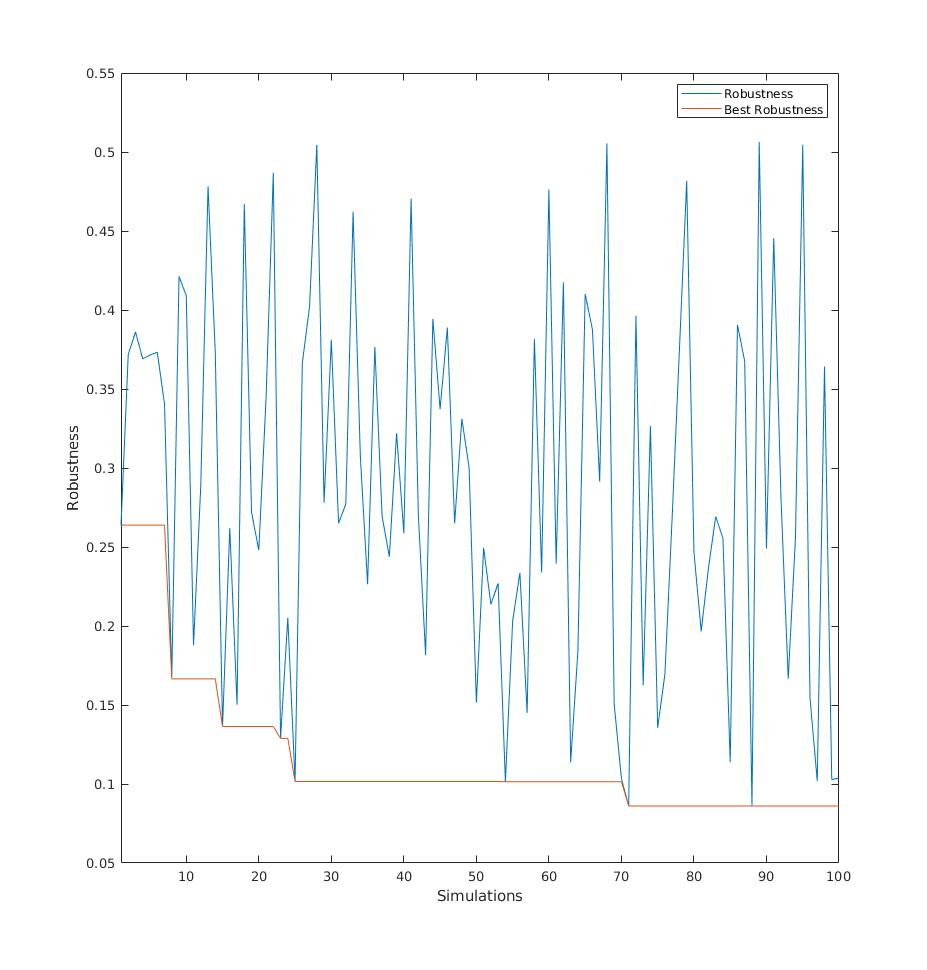
\includegraphics[width=0.5\linewidth]{img/urs_rob_distr.jpg}
    \caption{Robustness distribution over 100 simulation of URS search. This random distribution highlights that there is no learning in URS. Moreover, all the values are in [0,1] because we are using the normalized version of specific \texttt{S2} and is rather likely to reach the third gear at least once during the simulation with random values.}
\end{figure}

\subsection{Experiments}
detail of each experiment

\pagebreak

\section{Analysis of the results}
Oveerview of the different test, how many times and the difficutly overcomed (e.g., matlab poor randomness, o.o. poor peerformances and not correctness)

\subsection{Comments}
table with results and plot for robustnes and graph

\subsection{Hyperparameters}
General choises of C, region and quantization vs brancing factor

link to saved workspaces

\section{Conclusion}

\bibliographystyle{plain}
\bibliography{biblio}

\end{document}
